% bei Standalone in documentclass noch:
% \RequirePackage{luatex85}

\documentclass[captions=tableheading, titlepage= firstiscover, parskip = half , bibliography=totoc]{scrartcl}
%paper = a5 für andere optinen
% titlepage= firstiscover
% bibliography=totoc für bibdateien
% parskip=half  Veränderung um Absätze zu verbessern

\usepackage{scrhack} % nach \documentclass
\usepackage[aux]{rerunfilecheck}
\usepackage{polyglossia}
\usepackage[style=numeric, backend=biber]{biblatex} % mit [style = alphabetic oder numeric] nach polyglossia
\addbibresource{lit.bib}
\setmainlanguage{german}

\usepackage[autostyle]{csquotes}
\usepackage{amsmath} % unverzichtbare Mathe-Befehle
\usepackage{amssymb} % viele Mathe-Symbole
\usepackage{mathtools} % Erweiterungen für amsmath
\usepackage{fontspec} % nach amssymb
% muss ins document: \usefonttheme{professionalfonts} % für Beamer Präsentationen
\usepackage{longtable}

\usepackage[
math-style=ISO,    % \
bold-style=ISO,    % |
sans-style=italic, % | ISO-Standard folgen
nabla=upright,     % |
partial=upright,   % /
]{unicode-math} % "Does exactly what it says on the tin."
\setmathfont{Latin Modern Math}
% \setmathfont{Tex Gyre Pagella Math} % alternativ

\usepackage[
% die folgenden 3 nur einschalten bei documenten
locale=DE,
separate-uncertainty=true, % Immer Fehler mit ±
per-mode=symbol-or-fraction, % m/s im Text, sonst \frac
]{siunitx}

% alternativ:
% per-mode=reciprocal, % m s^{-1}
% output-decimal-marker=., % . statt , für Dezimalzahlen

\usepackage[
version=4,
math-greek=default,
text-greek=default,
]{mhchem}

\usepackage[section, below]{placeins}
\usepackage{caption} % Captions schöner machen
\usepackage{graphicx}
\usepackage{grffile}
\usepackage{subcaption}

% \usepackage{showframe} Wenn man die Ramen sehen will

\usepackage{float}
\floatplacement{figure}{htbp}
\floatplacement{table}{htbp}

\usepackage{mhchem} %chemische Symbole Beispiel: \ce{^{227}_{90}Th+}


\usepackage{booktabs}

 \usepackage{microtype}
 \usepackage{xfrac}

 \usepackage{expl3}
 \usepackage{xparse}

 % \ExplSyntaxOn
 % \NewDocumentComman \I {}  %Befehl\I definieren, keine Argumente
 % {
 %    \symup{i}              %Ergebnis von \I
 % }
 % \ExplSyntaxOff

 \usepackage{pdflscape}
 \usepackage{mleftright}

 % Mit dem mathtools-Befehl \DeclarePairedDelimiter können Befehle erzeugen werden,
 % die Symbole um Ausdrücke setzen.
 % \DeclarePairedDelimiter{\abs}{\lvert}{\rvert}
 % \DeclarePairedDelimiter{\norm}{\lVert}{\rVert}
 % in Mathe:
 %\abs{x} \abs*{\frac{1}{x}}
 %\norm{\symbf{y}}

 % Für Physik IV und Quantenmechanik
 \DeclarePairedDelimiter{\bra}{\langle}{\rvert}
 \DeclarePairedDelimiter{\ket}{\lvert}{\rangle}
 % <name> <#arguments> <left> <right> <body>
 \DeclarePairedDelimiterX{\braket}[2]{\langle}{\rangle}{
 #1 \delimsize| #2
 }

\setlength{\delimitershortfall}{-1sp}

 \usepackage{tikz}
 \usepackage{tikz-feynman}

 \usepackage{csvsimple}
 % Tabellen mit \csvautobooktabular{"file"}
 % muss in table umgebung gesetzt werden


% \multicolumn{#Spalten}{Ausrichtung}{Inhalt}

\usepackage{hyperref}
\usepackage{bookmark}
\usepackage[shortcuts]{extdash} %nach hyperref, bookmark

\newcommand{\ua}[1]{_\symup{#1}}
\newcommand{\su}[1]{\symup{#1}}


\begin{document}

\section{Auswertung}

Im Folgendem werden die Messergebnisse ausgewertet und in geeigneter
Weise visualisert.

\subsection{Grezfrequenzen}

Die verwendete Apparatur hatte die folgenden Werte.

\begin{align}
  \label{L}
  L &= \SI{1,217}{\milli\henry}\\
  \label{C_1}
  C_1 &= \SI{20,13}{\nano\farad}\\
  \label{C_2}
  C_2 &= \SI{9,41}{\nano\farad}
\end{align}

Diese Daten wurden ohne Fehler angegeben und werden deshalb als fehlerfrei
angenommen. In der $LC$-Kettenschaltung wurde der Kondensator mit der
Kapazität $C_1$ verwendet.

Mittels der Formeln ????? ergeben dich die die Grenzfrequenzen zu:

\begin{align*}
  \omega_{Grenz,C} &= \Si{404075,78}\frac{1}{\si{\second}}\\
  \omega_{Grenz,C_1C_2}^{akkustisch} &= \Si{285724,72}\frac{1}{\si{\second}}\\
  \omega_{Grenz,C_1C_2}^{optisch} &= \Si{417902,43}\frac{1}{\si{\second}}
\end{align*}

Mit Hilfe des $XY$-Scheibers wurden die Grenzfrequenzen der $LC$-Kettenschaltung
und der $LC_1C_2$-Kettenschaltung visualisiert. Die Diagramme sind
logarithmisch. Durch ermitteln der Frequenzen an bestimmten Stellen der
Grafik kann eine Exponentielle Regressionsrechnung gemacht werden.
Damit ist einen Zusammenhang zwischen den Messdaten und vom Generator durchlaufenden
Frequenzen bekannt.

Die Ausgleichsrechnung wurde mithilfe des \emph{Python}-Packetes
\emph{curve_Fit} bewerkstelligt. Die Funktion hatte die Gestalt.

\begin{equation}
  \nu(t) = a\cdot e^{bx}+c
\end{equation}

Es ergeben sich mittels der Messdaten (??) die folgenden Funktionen.

\begin{align}
  \label{eqn:Ausgleichsrechnung_exp}
  \nu_{C}(x) &= (13984\pm 1701)\cdot e^{(0,08\pm 0,005)\cdot x} - (5155\pm 2006) \\
  \nu_{C_1C_2}(x) &= (64117\pm 5474)\cdot e^{(0,15\pm 0,005)\cdot x}-(20547\pm 7703)
\end{align}

Anhand der Graphen kann die Grenzfrequenz abgelesen werden, indem der
Abstand vermessen wird. Das Messung wurde mit einem Lineal gemacht
und ergibt für die $LC$-Kettenschaltung einen Wert von ca.
$17,2 \si{\centi\meter}$. Die Messung der Grenzfrequenzen der
$LC_1C_2$-Kettenschaltung ergab für den akustischen Zweig eine
Grezfrequenz bei $11 \si{\centi\meter}$ und für den optischen Zweig eine
Grenzfrequenz bei  $12,2 \si{\centi\meter}$.

Für die Grenzfrequenzen ergeben sich damit die Werte:

\begin{align}
  \omega_{Grenz,C} &= \Si{50224,00\pm 3864,40}\frac{1}{\si{\second}}\\
  \omega_{Grenz,C_1C_2}^{akkustisch} &= \Si{311361,75\pm 13506,32}\frac{1}{\si{\second}}\\
  \omega_{Grenz,C_1C_2}^{optisch} &= \Si{376566,51\pm 13543,23}\frac{1}{\si{\second}}
\end{align}

\section{Dispersionskurven}

Mit den Angaben \eqref{L}, \eqref{C_1} und \eqref{C_2} kann die Dispersionskurve_C1C2_2
der $LC-Kette$ und der $LC_1C_2$-Kette über die Funktion (??) bestimmt werden.
Die Messdaten wurden in das Diagramm mit eingetragen.

\begin{figure}
  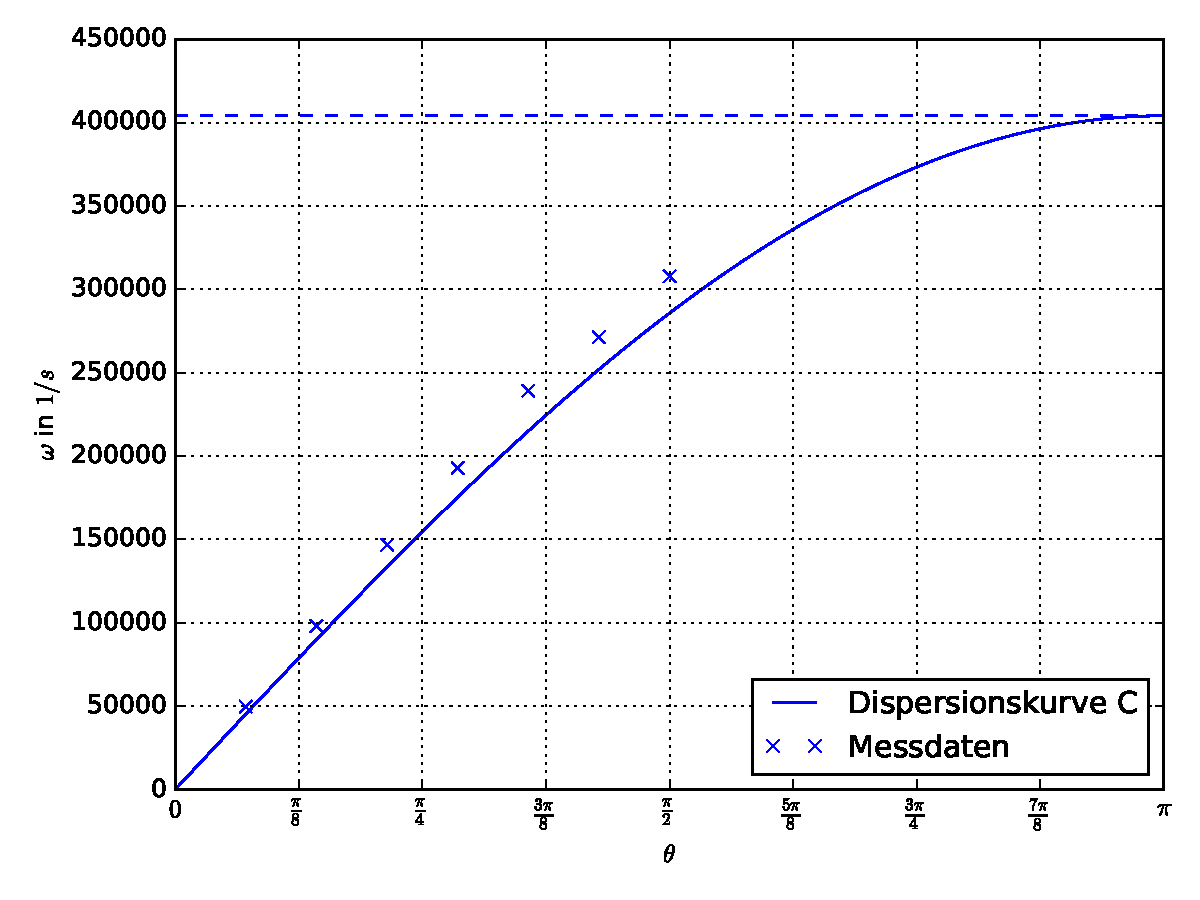
\includegraphics[width=\textwidth]{Dispersionskurve_C.pdf}
  \caption{Dispersionskurve der $LC$-Kettenschaltung}
  \label{fig:Dispersion_C}
\end{figure}
\begin{figure}
  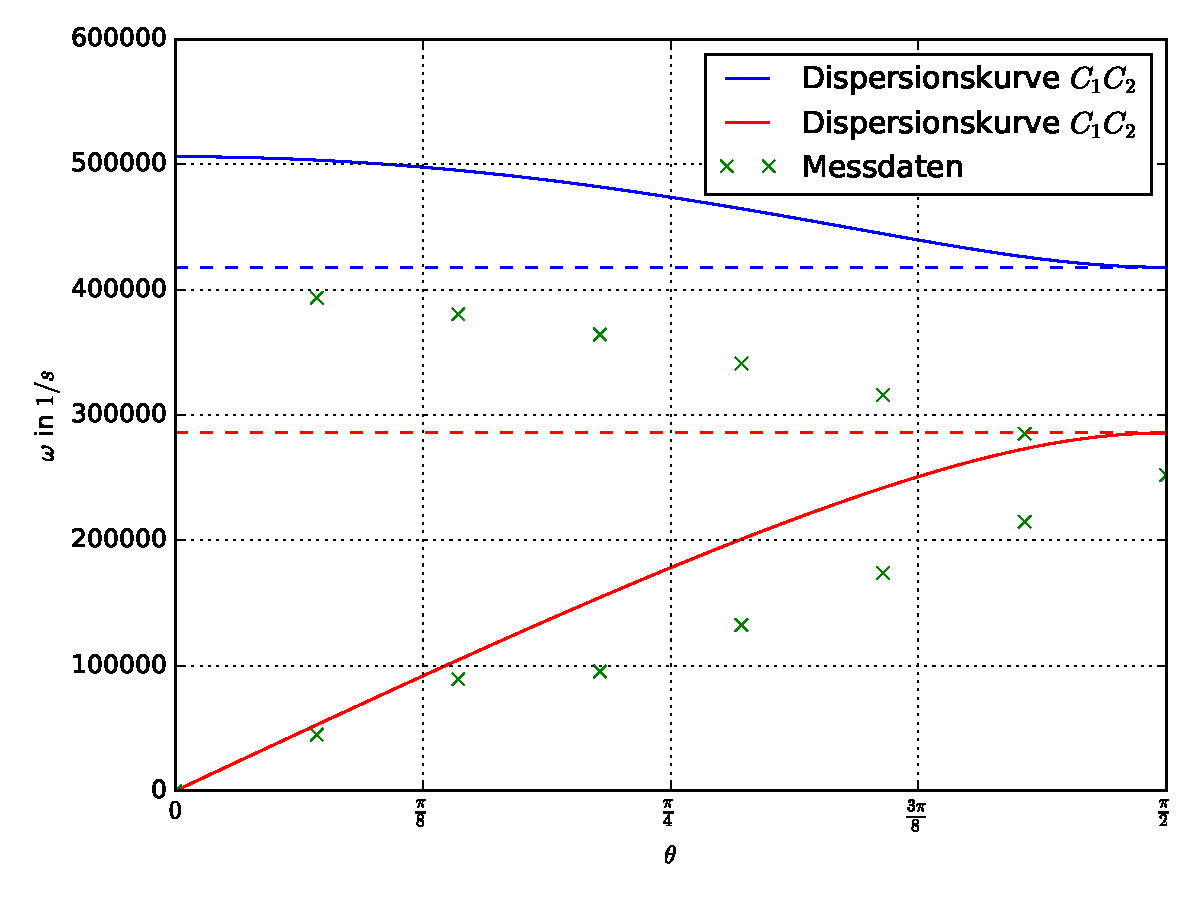
\includegraphics[width=\textwidth]{Dispersionskurve_C1C2.pdf}
  \caption{Dispersionskurve der $LC_1C_2$-Kettenschaltung}
  \label{fig:Dispersion_C1C2}
\end{figure}

\subsection{Stehende Wellen}

Beim messen der Spannungsamplituden der offenen $LC$-Kette ergeben sich die folgenden
Diagramme.

\begin{figure}
  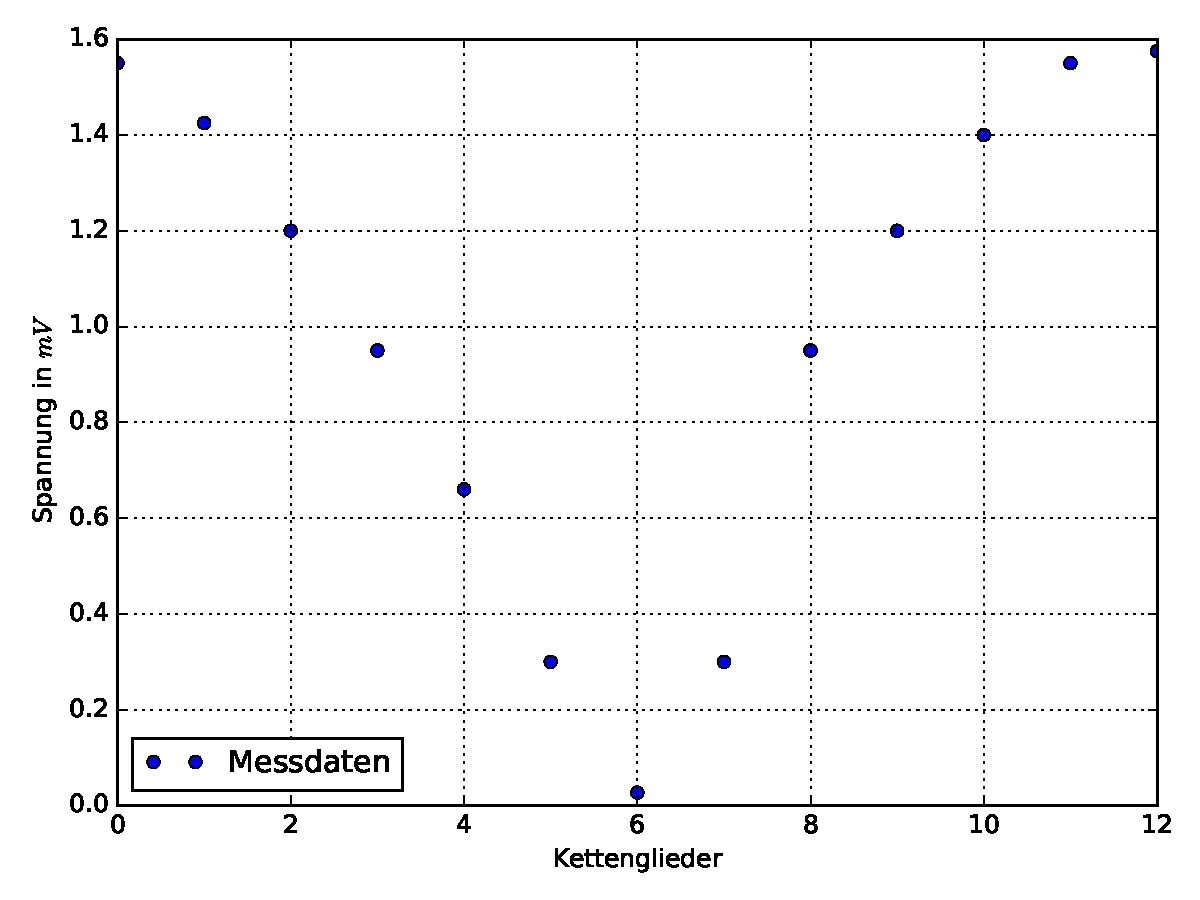
\includegraphics[width=\textwidth]{Messung_d_1.pdf}
  \caption{Erste Grundschwingung der offenen $LC$-Kettenschaltung}
  \label{fig:Messung_d_1
\end{figure}

\begin{figure}
  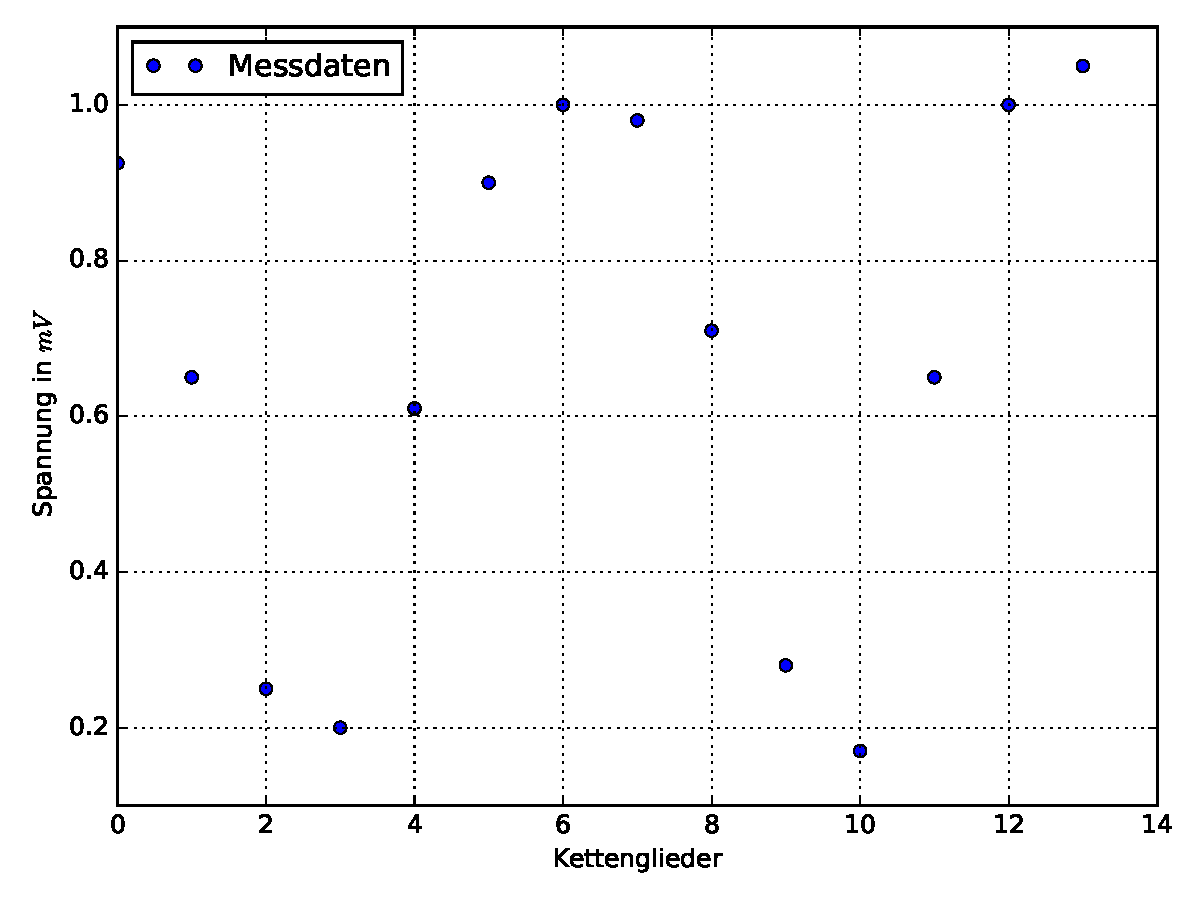
\includegraphics[width=\textwidth]{Messung_d_2.pdf}
  \caption{Zweite Grundschwingung der offenen $LC$-Kettenschaltung}
  \label{fig:Messung_d_2}
\end{figure}

\begin{figure}
  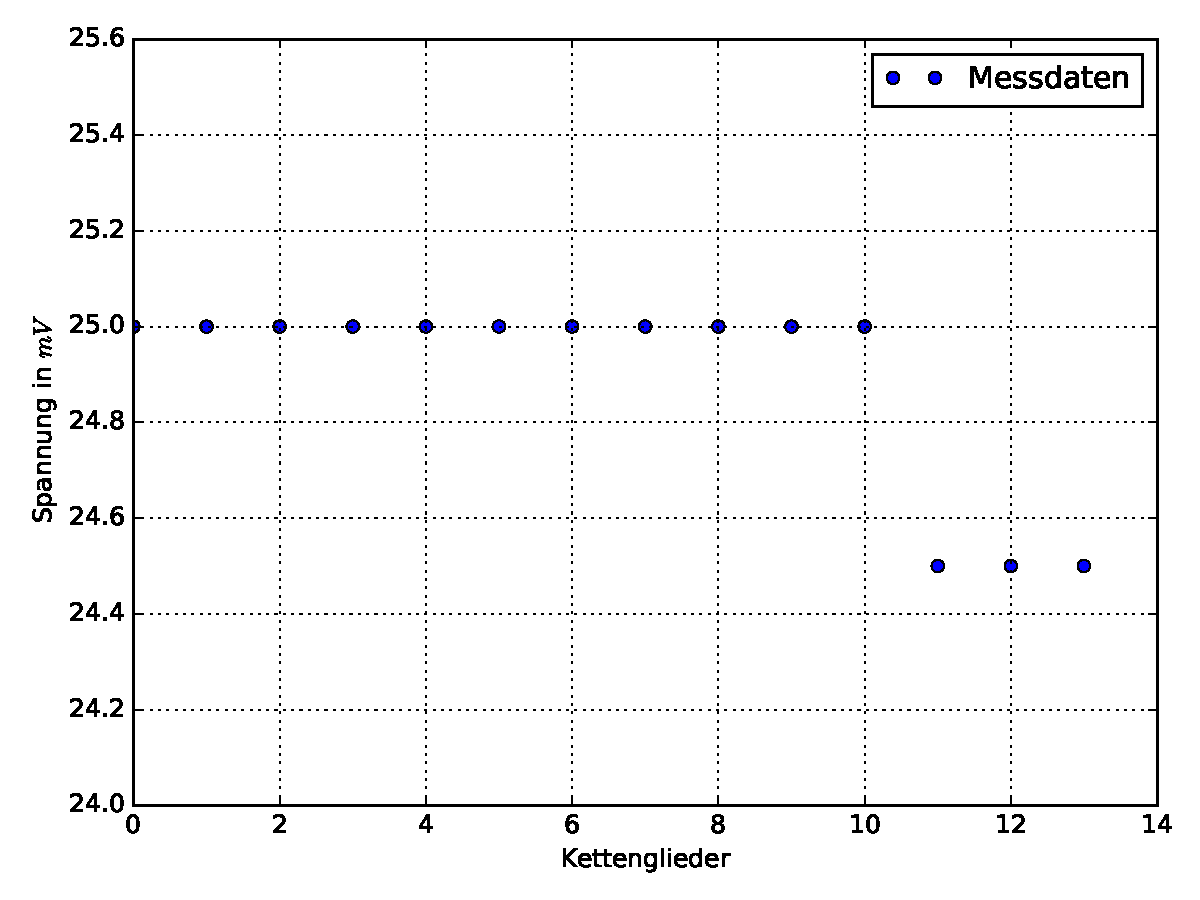
\includegraphics[width=\textwidth]{Messung_e.pdf}
  \caption{Abgeschlossene $LC-$Kettenschaltung}
  \label{fig:Messung_e}
\end{figure}

\end{document}
